\section{Example}

A typical usage of this package is to pre-process a point set before calling a reconstruction method.
Surface Reconstruction from Point Sets is a sequential process:

\begin{itemize}
\item Scanning and scan alignment produce a set of points
      or points with normals. Alignment is not yet
      covered by \cgal.
\item Outlier removal for reconstruction methods which
      are not resilient to outliers.
\item Simplification to reduce the number of input points.
\item Smoothing to reduce noise in the input data.
\item Normal estimation and orientation when the normals
      are not already provided by the acquisition device.
\item Surface reconstruction.
\end{itemize}

\cgal\ provides algorithms for all steps listed above except alignment.\\
This package provides outlier removal, simplification, smoothing,
normal estimation and orientation.\\
Chapter \ccc{Surface_reconstruction_points_3} \ref{chap:surface_reconstruction_points_3}
describes surface reconstruction using \cgal\ Surface Mesh Generator.

% Insert image pipeline.jpg/eps
\begin{center}
    \label{Point_set_processing_3-fig-pipeline}
    % Image
    \begin{ccTexOnly}
        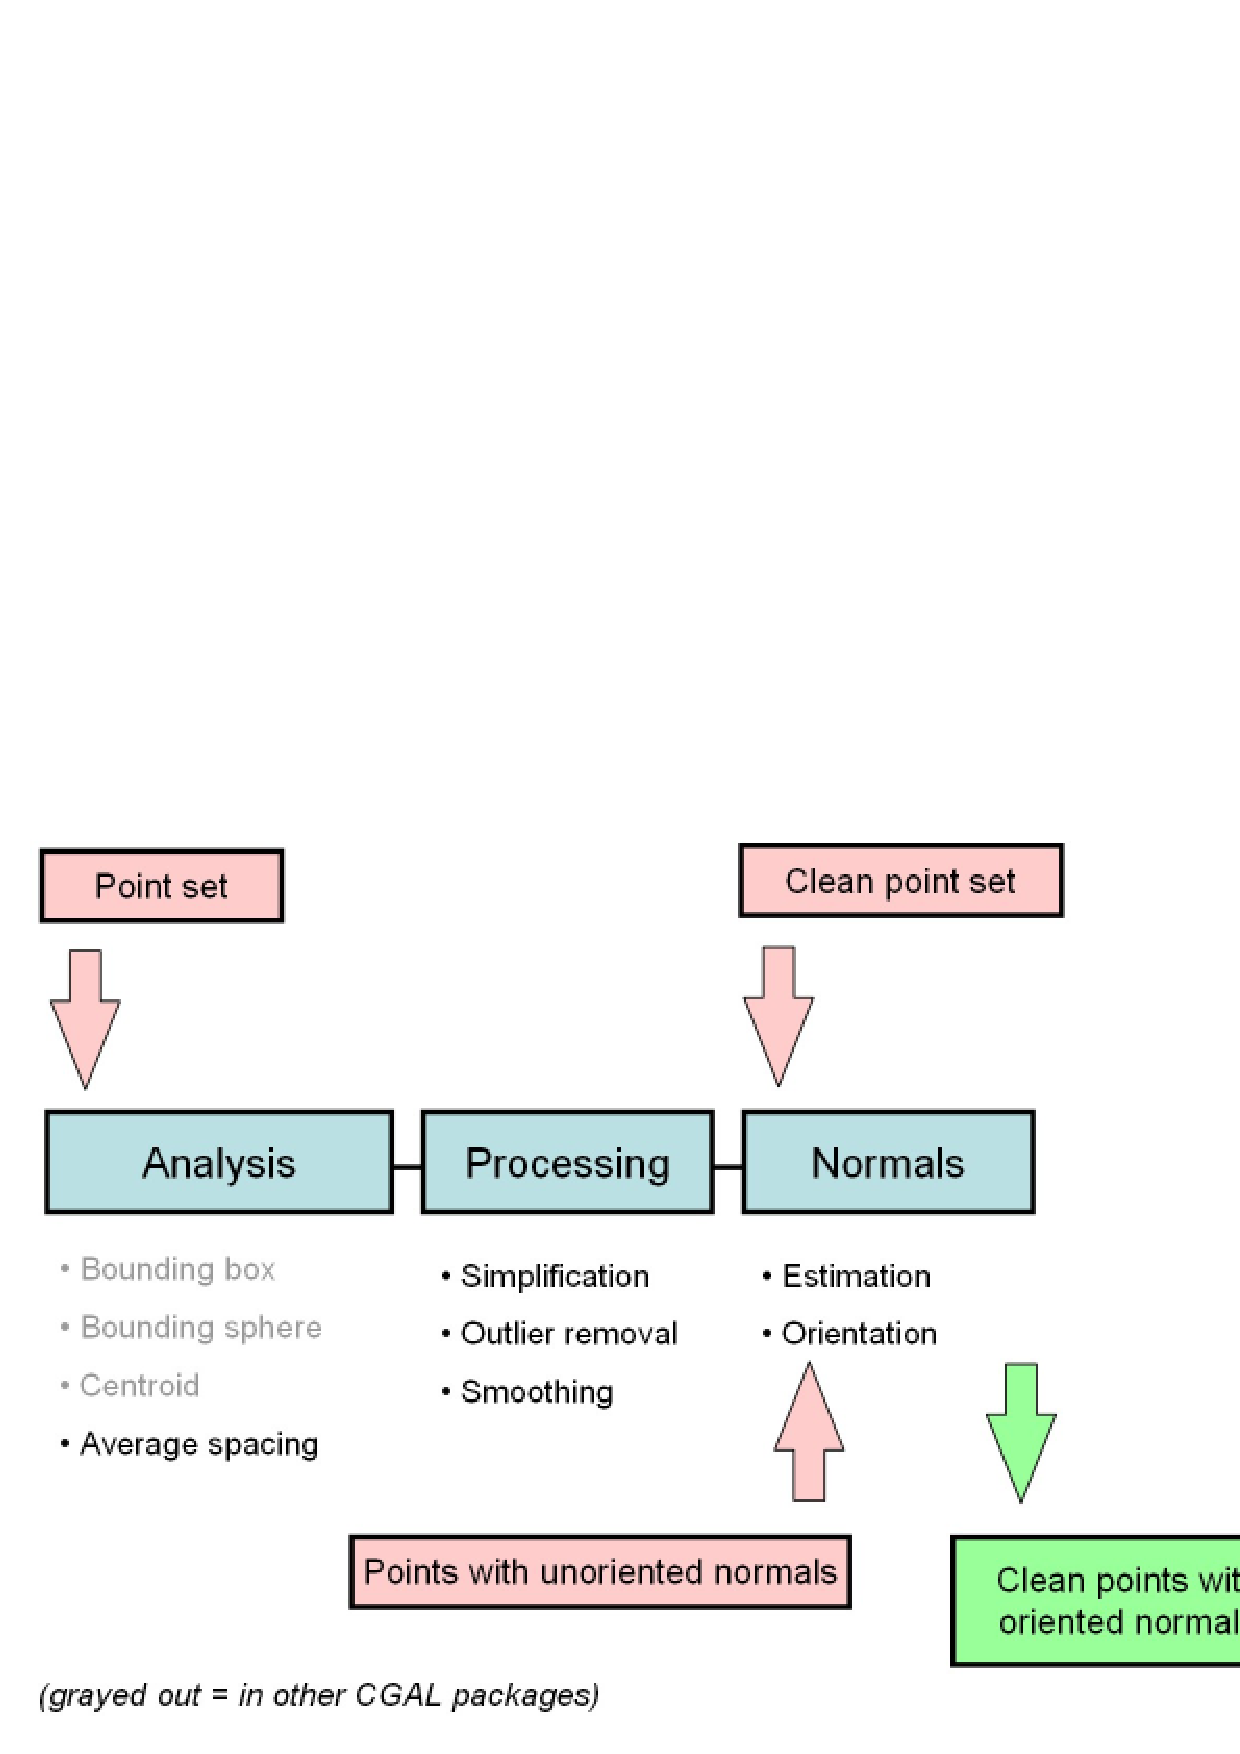
\includegraphics[width=0.8\textwidth]{Point_set_processing_3/pipeline} % omit .eps suffix
    \end{ccTexOnly}
    \begin{ccHtmlOnly}
        <img width="65%" border=0 src="./pipeline.jpg"><P>
    \end{ccHtmlOnly}
    % Title
    \begin{figure}[h]
        \caption{Point Set Processing pipeline.}
    \end{figure}
\end{center}


\section{Input}

The algorithms of this component expect as input parameters range iterators over:

\begin{itemize}
\item 3D points
\item Normals (orientable 3D vectors)
\item 3D points with unoriented normals
\item 3D points with oriented normals
\end{itemize}

These types are described as concepts.
\cgal\ provides the next classes to implement points and normals:

\begin{itemize}
\item \ccRefIdfierPage{CGAL::Point_3<GeomTraits>} \\
\cgal\ 3D position.
\item \ccRefIdfierPage{CGAL::Vector_3<GeomTraits>} \\
\cgal\ 3D vector.
\item \ccRefIdfierPage{CGAL::Orientable_normal_3<GeomTraits>} \\
Normal (oriented or not). Inherits from \ccc{Vector_3<GeomTraits>} and contains an additional orientation flag.
\item \ccRefIdfierPage{CGAL::Point_with_normal_3<GeomTraits, Normal_3>} \\
3D point location plus normal.
\end{itemize}

We provide convenient functions to read point sets from standard file formats:

\begin{itemize}
\item XYZ
\item OFF
\end{itemize}

\ccRefIdfierPage{CGAL::read_xyz_point_set}  \\
\ccRefIdfierPage{CGAL::read_off_point_set}  \\

Example:

\ccIncludeExampleCode{Point_set_processing_3/read_write_xyz_point_set_example.cpp}


\section{Analysis}

The purpose of the analysis stage is to measure common statistics and bounding volumes over the input points so as to automatically determine parameters for subsequent stages:
\begin{itemize}
  \item Point set barycenter, bounding box,
        bounding sphere (provided by other \cgal\ components).
  \item Average spacing to the $k$ nearest neighbors.
\end{itemize}

\ccc{CGAL::average_spacing_3()} computes the average spacing of all input points to their $k$ nearest neighbors.

\ccRefIdfierPage{CGAL::centroid}  \\
\ccRefIdfierPage{CGAL::bounding_box}  \\
\ccRefIdfierPage{CGAL::bounding_sphere}  \\
\ccRefIdfierPage{CGAL::average_spacing_3}  \\

Example:

\ccIncludeExampleCode{Point_set_processing_3/average_spacing_example.cpp}


\section{Outlier Removal}

Function \ccc{CGAL::outlier_removal_3()} deletes a user-specified fraction of outliers from the input point set. More specifically, it sorts the input points in increasing order of average squared distances to the $k$ nearest neighbors and deletes the points with largest value.

\emph{Note to the reviewers: we will add a function in the analysis section which displays in the console the distribution of such average squared distance so as to help the user picking an appropriate fraction value.}

\ccRefIdfierPage{CGAL::outlier_removal_3}  \\

% % Insert image outlier_removal.jpg/eps
% \begin{center}
%     \label{Point_set_processing_3-fig-outlier_removal}
%     % Image
%     \begin{ccTexOnly}
%         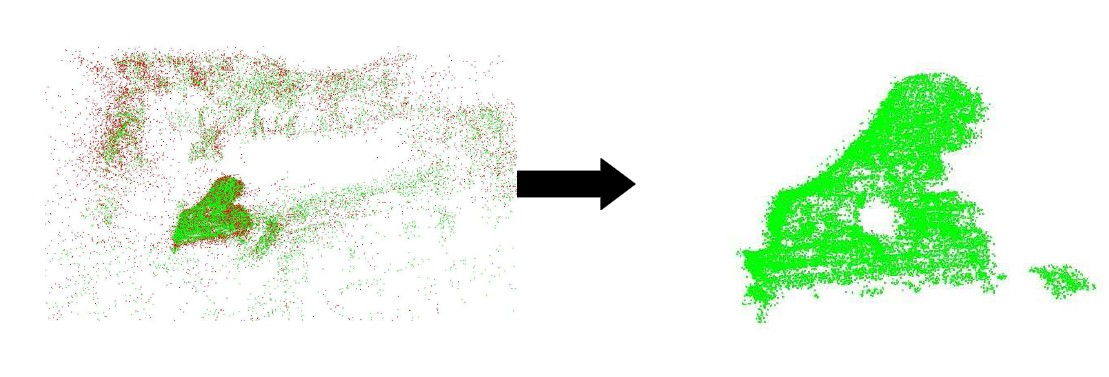
\includegraphics[width=0.9\textwidth]{Point_set_processing_3/outlier_removal} % omit .eps suffix
%     \end{ccTexOnly}
%     \begin{ccHtmlOnly}
%         <img width="90%" border=0 src="./outlier_removal.jpg"><P>
%     \end{ccHtmlOnly}
%     % Title
%     \begin{figure}[h]
%         \caption{Outlier removal}
%     \end{figure}
% \end{center}

Example:

\ccIncludeExampleCode{Point_set_processing_3/outlier_removal_example.cpp}


\section{Simplification}

Two functions are provided to simplify the input point set.

\ccc{CGAL::merge_simplification_3()} iteratively merges pairs of points which are epsilon-closed.\\
This algorithm is precise but slower than \ccc{CGAL::random_simplification_3()}.

\ccc{CGAL::random_simplification_3()} randomly deletes a user-specified fraction of points from the input point set.\\
This algorithm is very fast.

\ccRefIdfierPage{CGAL::merge_simplification_3}  \\
\ccRefIdfierPage{CGAL::random_simplification_3}  \\

% Insert image merge_simplification.jpg/eps
\begin{center}
    \label{Point_set_processing_3-fig-merge_simplification}
    % Image
    \begin{ccTexOnly}
        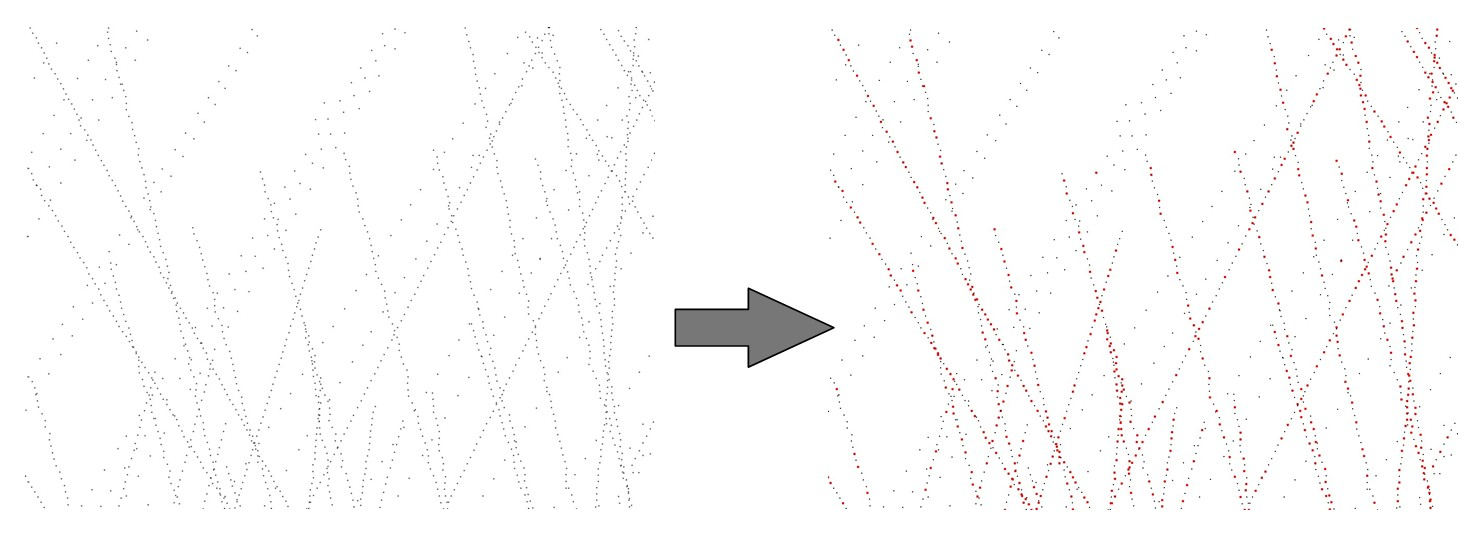
\includegraphics[width=1.0\textwidth]{Point_set_processing_3/merge_simplification} % omit .eps suffix
    \end{ccTexOnly}
    \begin{ccHtmlOnly}
        <img width="100%" border=0 src="../Point_set_processing_3/merge_simplification.jpg"><P>
    \end{ccHtmlOnly}
    % Title
    \begin{figure}[h]
        \caption{Point set simplification by merging.
                 Left: input point set.
                 Right: removed points are depicted in red.}
    \end{figure}
\end{center}

Example:

\ccIncludeExampleCode{Point_set_processing_3/random_simplification_example.cpp}


\section{Smoothing}

Function \ccRefIdfierPage{CGAL::jet_smoothing_3} smooths the input point set by projecting each point onto a smooth parametric surface patch (so-called jet surface) fitted over the $k$ nearest neighbors. \\

% % Insert image jet_smoothing.jpg/eps
% \begin{center}
%     \label{Point_set_processing_3-fig-jet_smoothing}
%     % Image
%     \begin{ccTexOnly}
%         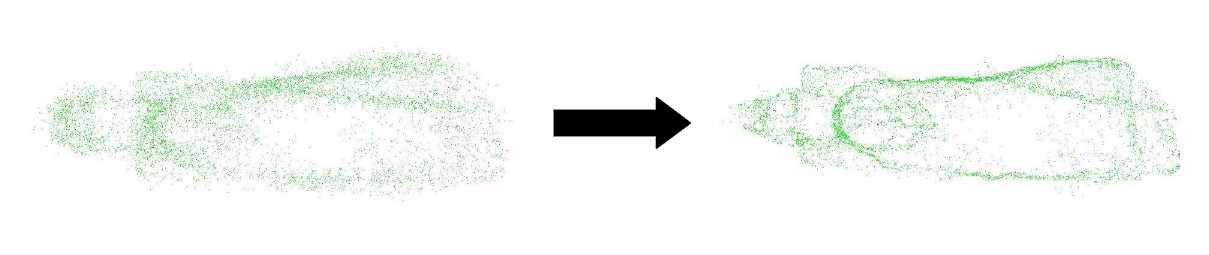
\includegraphics[width=1.0\textwidth]{Point_set_processing_3/jet_smoothing} % omit .eps suffix
%     \end{ccTexOnly}
%     \begin{ccHtmlOnly}
%         <img width="100%" border=0 src="./jet_smoothing.jpg"><P>
%     \end{ccHtmlOnly}
%     % Title
%     \begin{figure}[h]
%         \caption{Point set smoothing}
%     \end{figure}
% \end{center}

Example:

\ccIncludeExampleCode{Point_set_processing_3/jet_smoothing_example.cpp}


\section{Normal Estimation}

Two functions are provided to estimate the normal direction of the inferred surface at each point from the input point set. In both cases, the result is an unoriented normal vector for each input point.

Function \ccc{CGAL::jet_normal_estimation()} estimates the normal direction at each point from the set by fitting a jet surface over its $k$ nearest neighbors. The default jet is a quadric surface.\\
This algorithm is well suited to point sets scattered over curved surfaces.

Function \ccc{CGAL::pca_normal_estimation()} estimates the normal direction at each point from the set by linear least squares fitting of a plane over its $k$ nearest neighbors.\\
This algorithm is well suited to point sets scattered over plane surfaces. It is much faster than \ccc{CGAL::jet_normal_estimation()}.

\ccRefIdfierPage{CGAL::pca_normal_estimation}  \\
\ccRefIdfierPage{CGAL::jet_normal_estimation}  \\

% % Insert image pca_normal_estimation.jpg/eps
% \begin{center}
%     \label{Point_set_processing_3-fig-pca_normal_estimation}
%     % Image
%     \begin{ccTexOnly}
%         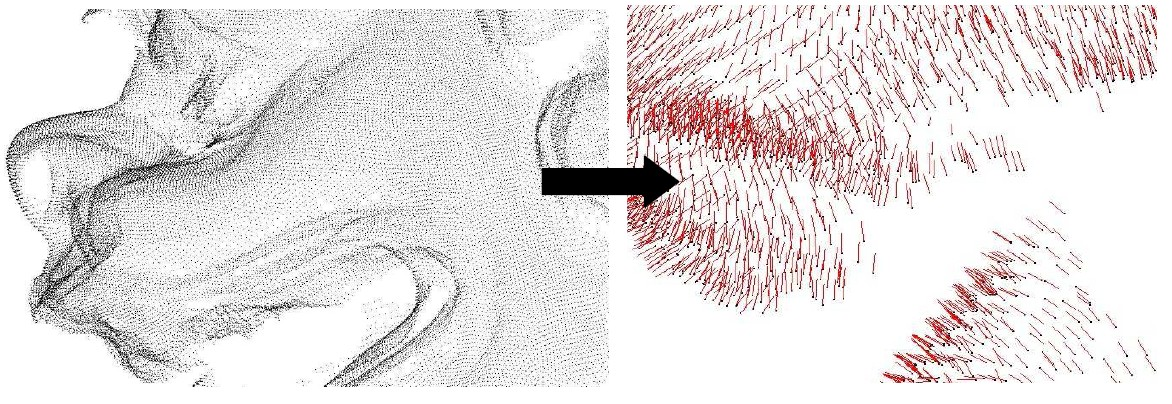
\includegraphics[width=0.9\textwidth]{Point_set_processing_3/pca_normal_estimation} % omit .eps suffix
%     \end{ccTexOnly}
%     \begin{ccHtmlOnly}
%         <img width="90%" border=0 src="./pca_normal_estimation.jpg"><P>
%     \end{ccHtmlOnly}
%     % Title
%     \begin{figure}[h]
%         \caption{Normal estimation by Principal Components Analysis}
%     \end{figure}
% \end{center}

Example:

\ccIncludeExampleCode{Point_set_processing_3/pca_normal_estimation_example.cpp}


\section{Normal Orientation}

Function \ccc{CGAL::mst_normal_orientation()} orients the normals of a set of points with (unoriented) normals using the method described by Hoppe et al. in {\em Surface reconstruction from unorganized points} \cite{cgal:hddms-srup-92}. More specifically, this method constructs a Riemannian graph over the input points and propagates a seed normal orientation within a minimum spanning tree computed over the graph with the Boost graph library. The result is an oriented normal vector for each input point/normal.

\ccRefIdfierPage{CGAL::mst_normal_orientation}  \\

% Insert image mst_normal_orientation.jpg/eps
\begin{center}
    \label{Point_set_processing_3-fig-mst_normal_orientation}
    % Image
    \begin{ccTexOnly}
        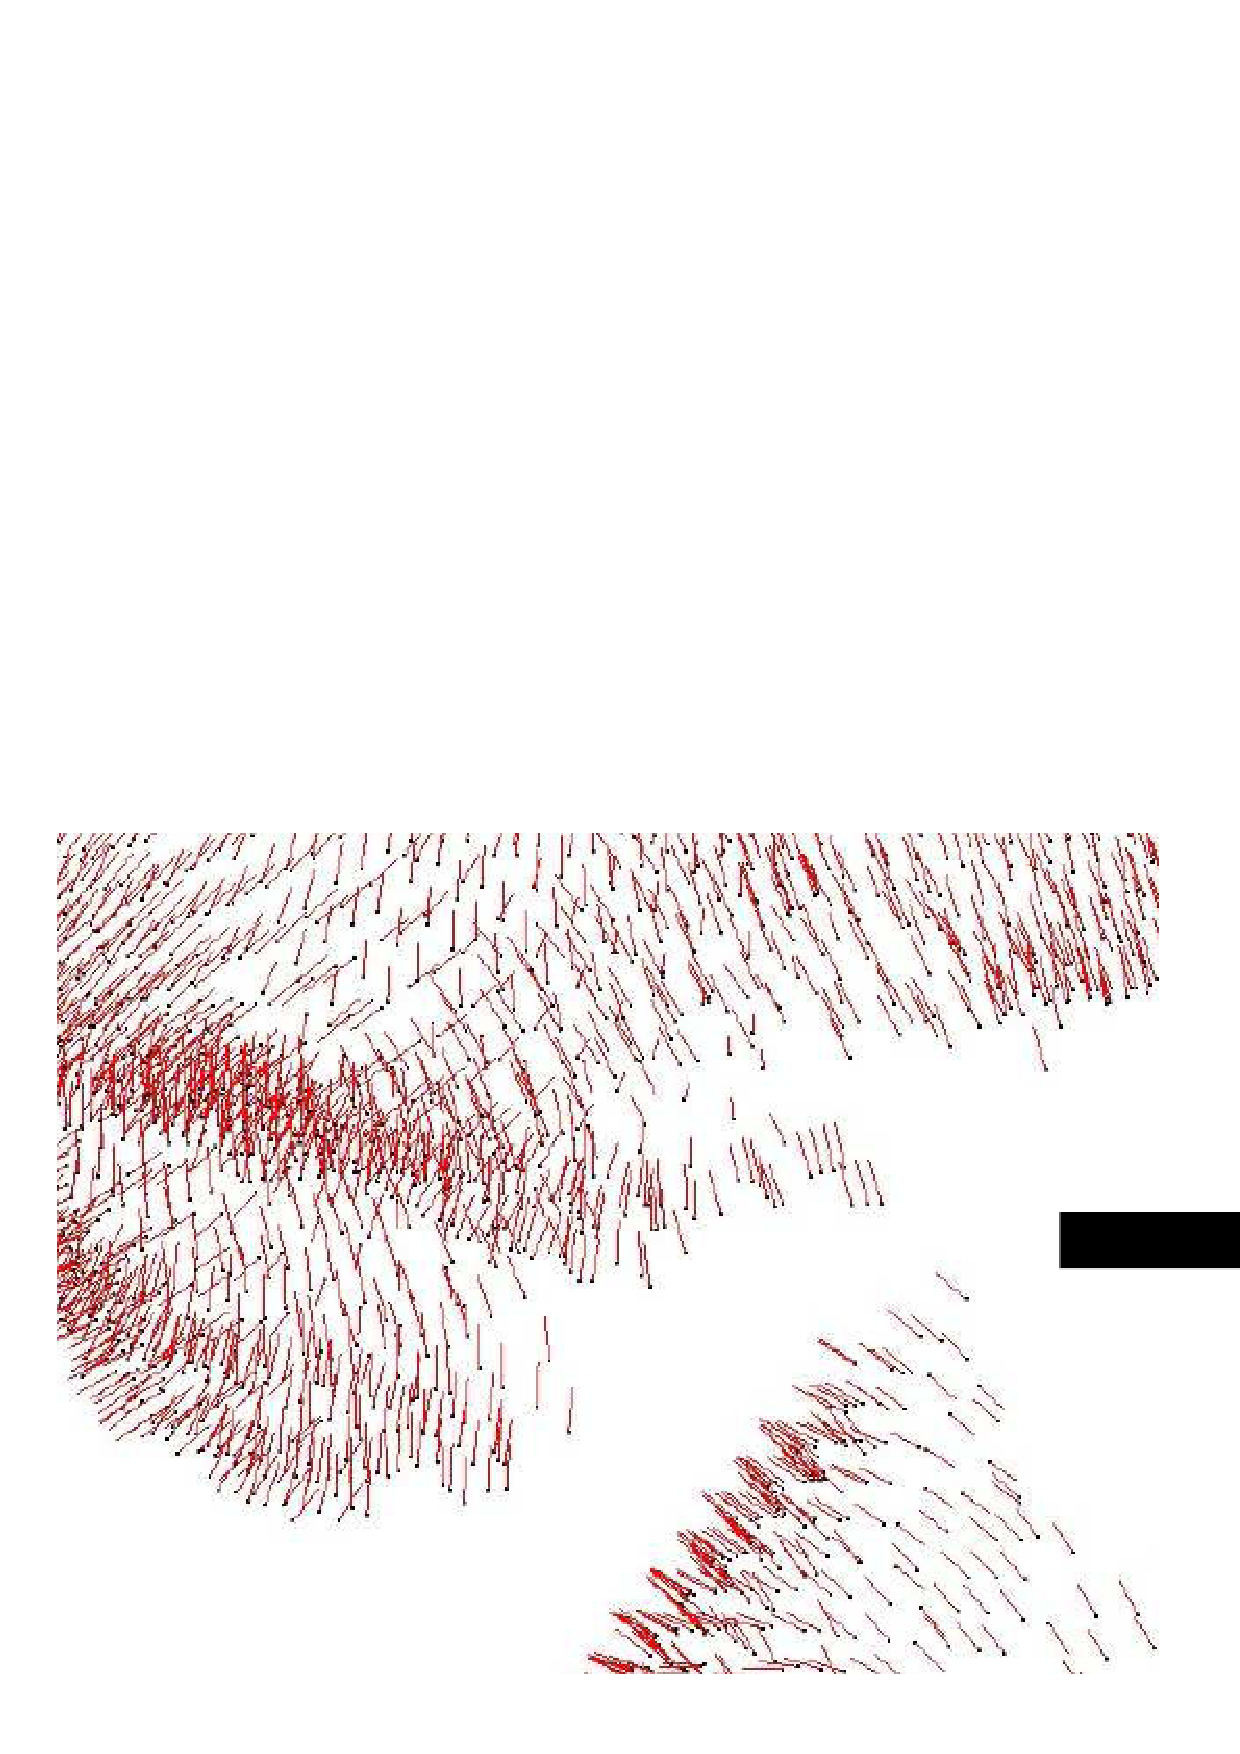
\includegraphics[width=1.0\textwidth]{Point_set_processing_3/mst_normal_orientation} % omit .eps suffix
    \end{ccTexOnly}
    \begin{ccHtmlOnly}
        <img width="100%" border=0 src="./mst_normal_orientation.jpg"><P>
    \end{ccHtmlOnly}
    % Title
    \begin{figure}[h]
        \caption{Normal orientation of a cube's normals. Notice the left and bottom normals orientation.}
    \end{figure}
\end{center}

Example: see \ccc{pca_normal_estimation_example.cpp} example above.


\section{Output}

The output of the processing stage is a point set with normals.
For convenience, we provide functions to write point sets to standard file formats:
\begin{itemize}
\item XYZ
\item OFF
\end{itemize}

\ccRefIdfierPage{CGAL::write_off_point_set}  \\
\ccRefIdfierPage{CGAL::write_xyz_point_set}  \\

Example:

See \ccc{read_write_xyz_point_set_example.cpp} example above.

